\documentclass{../notatki}

\title{Wprowadzenie do teorii sieci neuronowych}

\begin{document}

\tableofcontents

\section{Model McCullocha-Pittsa}

Jest to model matematyczny mający naśladować działanie fizjologicznych neuronów.
Składa się on z $n$ wejść $u_i$ o wagach $w_i$ i jednego wyjścia $y$.
Neuron aktywuje się, gdy suma iloczynów wejść i wag jest większa od
pewnej wartości progowej $\theta$.
$$
n_i,y \in \{0.0, 1.0\} \subset \mathbb{R}
$$
$$
w_i, \theta \in \mathbb{R}
$$
$$
f(x) =
\begin{cases}
  0 & x < 0\\
  1 & x \geq 0
\end{cases}
$$
$$
y(\vec{u}, \vec{w}) = f((\sum_{i=1}^{n}w_iu_i) - \theta)
$$
\begin{figure*}[h]
  \centering
  \begin{tikzpicture}[node distance=0.7cm]
    \node[circle, draw=black] (neuron) {$f$};
    \node (u1) [above left=of neuron] {$u_{i + 1}$};
    \node (dots) [left=of neuron] {$\vdots$};
    \node (u2) [below left=of neuron] {$u_i$};
    \draw[->] (u1) -- (neuron) node[midway, right] {$w_{i + 1}$};
    \draw[->] (u2) -- (neuron) node[midway, right] {$w_i$};
    \draw[->] (neuron) -- ++(1, 0) node[right] {$y$};
  \end{tikzpicture}
  \caption{Wizualizacja modelu McCullocha-Pittsa}
\end{figure*}

\subsection{Przykład}

\begin{table}[h]
  \centering
  \begin{tabular}{|c|c|c|c|}
    \hline
    $u_1$ & $u_2$ & $y$\\
    \hline
    0 & 0 & 0\\
    0 & 1 & 0\\
    1 & 0 & 0\\
    1 & 1 & 1\\
    \hline
  \end{tabular}
  \caption{Tabela prawdy dla funkcji logicznej AND}
\end{table}

\begin{itemize}
  \item $u_1 = u_2 = 0 \rightarrow y = 0 = f(-\theta) \leftrightarrow
    \theta \geq 0$
  \item $u_1 = 0, u_2 = 1 \rightarrow y = 0 = f(w_2 - \theta)
    \leftrightarrow w_2 < \theta$
  \item $u_1 = 1, u_2 = 0 \rightarrow y = 0 = f(w_1 - \theta)
    \leftrightarrow w_1 < \theta$
  \item $u_1 = u_2 = 1 \rightarrow y = 1 = f(w_1 + w_2 - \theta)
    \leftrightarrow w_1 + w_2 \geq \theta$
\end{itemize}

$$
\theta = 3, w_1 = 2, w_2 = 2
$$

\subsection{Reprezentacja wektorowa}

$$
\vec{u} = (u_1, u_2, \ldots, u_n)
$$
$$
\vec{w} = (w_1, w_2, \ldots, w_n)
$$
$$
y(\vec{u}, \vec{w}) = f(\vec{w} \cdot \vec{u} - \theta)
$$

\section{Liniowa separowalność}

$$
U_- = \{\vec{u_1}, \dots, \vec{u_n}\} \subset \mathbb{R}^n
$$
$$
U_+ = \{\vec{v_{n + 1}}, \dots, \vec{v_{n + m}}\} \subset \mathbb{R}^n
$$
$$
U_- \cap U_+ = \emptyset
$$
Mówimy, że zbiory wektorów (wejść) $U_-$ i $U_+$ są liniowo separowalne, jeśli
istnieje jakikolwiek $\vec{w}$ taki, że: $\vec{w} \cdot \vec{u} < 0:
\vec{u} \in U_-$ oraz $\vec{w} \cdot \vec{u} > 0: \vec{u} \in U_+$. Innymi słowy
jeśli istnieje hiperpłaszczyzna, która dzieli zbiory $U_-$ i $U_+$.

\subsection{Przykład}

Dla bramki AND mamy:
$$
U_- = \{(0, 0), (0, 1), (1, 0)\}, U_+ = \{(1, 1)\}
$$

$$
\vec{w} = (2, 2), \theta = 3
$$

\begin{figure*}[h]
  \centering
  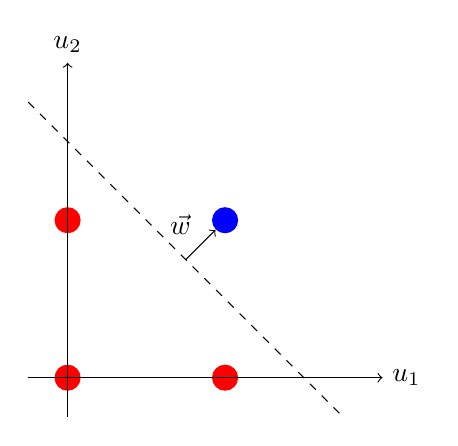
\begin{tikzpicture}
    \node[circle, fill=red, radius=0.1] (u1) at (0, 0) {};
    \node[circle, fill=red] (u2) at (0, 2) {};
    \node[circle, fill=red] (u3) at (2, 0) {};
    \node[circle, fill=blue] (v1) at (2, 2) {};
    \draw[->] (-0.5, 0) -- (4, 0) node[right] {$u_1$};
    \draw[->] (0, -0.5) -- (0, 4) node[above] {$u_2$};
    \draw[->] (1.5, 1.5) -- (v1) node[midway, above left] {$\vec{w}$};
    \draw[dashed] (-0.5, 3.5) -- (3.5, -0.5);
  \end{tikzpicture}
  \caption{Liniowa separowalność dla bramki AND}
\end{figure*}

\end{document}